\chapter{Z Tanım Bölgesinde PID Kontrolör Tasarımı}
\begin{enumerate}
    \item Geçici hal yanıtını şekillendirecek isterler dikkate alınarak s tanım bölgesinde baskın kutuplar seçilir. 
    \item Baskın kutuplar $z=e^{sT}$ ilişkisi ile z tanım bölgesine aktarılır. 
    \item Kontrol edilecek sistem Z tanım bölgesine geçirilir. 
    \item Kapalı çevrim transfer fonksiyonu elde edilir ve kutup atama yapılır.
\end{enumerate}
Örnek sistem
\begin{equation}
    G(s)=\frac{1}{s+2}
\end{equation}
z tanım bölgesinde $T=0.2$ olmak üzere
\begin{equation}
    G(z)=\frac{0.1648}{z-0.6703}
\end{equation}
olarak elde edilmektedir. Yerleşme zamanı $t_s=2$ ve aşım $\%10$ isterleri verilmiştir. Bu durumda $\zeta=0.591$ ve $w_n=6.7664$ seçilir. Seçilen sönüm oranı ve doğal frekans ile baskın kutuplar
\begin{equation}
    s_{1,2}=-4 \pm 5.4575i
\end{equation}
şeklinde hesaplanır. $z=e^{sT}$ ifadesi ile z tanım bölgesinde kutuplar
\begin{equation}
    z_{1,2}=0.2072 \pm 0.3987i
\end{equation}
ve kutuplardan oluşturulacak polinom
\begin{equation}
    p(z)=z^2-0.4144 z+0.2019
\end{equation}
olarak hesaplanır. PID kontrolör
\begin{equation}
\begin{split}
    F(z)&=K_p+\frac{K_iz}{z-1}+K_d\frac{z-1}{z}\\
    &=\frac{K_p(z^2-z)+K_iz^2+K_d(z-1)^2}{z^2-z}\\
    &=\frac{K_pz^2-K_pz+K_iz^2+K_dz^2-2K_dz+K_d}{z^2-z}\\
    &=\frac{(K_p+K_i+K_d)z^2-(K_p+2K_d)z+K_d}{z^2-z}
\end{split}
\end{equation}
olarak tanımlanmıştır. Kapalı çevrim transfer fonksiyonu
\begin{equation}
    \begin{split}
        T(z)&=\frac{F(z)G(z)}{1+F(z)G(z)}\\
        &=\frac{\frac{(K_p+K_i+K_d)z^2-(K_p+2K_d)z+K_d}{z^2-z}\frac{0.1648}{z-0.6703}}{1+\frac{(K_p+K_i+K_d)z^2-(K_p+2K_d)z+K_d}{z^2-z}\frac{0.1648}{z-0.6703}}\\
        &=\frac{0.1648((K_p+K_i+K_d)z^2-(K_p+2K_d)z+K_d)}{(z^2-z)(z-0.6703)+0.1648((K_p+K_i+K_d)z^2-(K_p+2K_d)z+K_d)}
    \end{split}
\end{equation}
olmaktadır. Bu durumda tasarım problemi
\begin{equation}
    \begin{split}
        0.1648(K_p+K_i+K_d)-1.6703&= p- 0.4144\\
        0.6703-0.1648(K_p+2K_d)&=0.2019 - 0.4144p\\
        0.1648K_d&=0.2019p
    \end{split}
\end{equation}
olarak verilir. Burada polinom dereceleri eşitlemek amacıyla tasarlanan polinom $s+p$ terimi ile çarpılmıştır. Görüldüğü üzere bilinmeyen sayısı denklem sayısından fazla olması sebebiyle birden çok çözüm bulunmaktadır. Bu durum bir fırsata çevrilirse, isterleri sağlama konusunda bir eniyileştirme işlemi yapılabilir. Bunun için parametrik çözüm elde edilmelidir. $p$, $k_d$ ve $k_i$ kalan parametre $k_p$ cinsinden elde edilirse 
\begin{equation}
    \begin{split}
        p&=15.51k_p-44.08\\
        k_d&=19k_p-54\\
        k_i&=74.1k_p-205.8
    \end{split}
\end{equation}
olarak bulunur. Kapalı çevrim sistemin kararlılığı açısından $|p|<1$ şartı sağlanmalıdır. Bu sebeple $k_p$ için sınır değerler
\begin{equation}
    15.51k_p-44.08=1,\quad 15.51k_p-44.08=-1
\end{equation}
denklemleri çözülerek 
\begin{equation}
    2.7778<k_p<2.9067
\end{equation}
elde edilir. Bu aralıkta değerler tek tek seçilir ve kapalı çevrim transfer fonksiyonu ve elde edilen yerleşme zamanı ve aşım verileri ile 
\begin{equation}
    J(k_p)=\frac{|t_s-1|}{2}+\frac{|os-10|}{20}
\end{equation}
amaç fonksiyonunda yerine yazılır. $J(k_p)$'yi en az yapan $k_p$ değeri $k_p=2.7998$ olarak elde edilir. Bu durumda kontrolör parametreleri $k_d=-0.8067$ ve $k_i=1.6319$ ve dolayısıyla kontrolör transfer fonksiyonu
\begin{equation}
    F(z)=\frac{3.625 z^2 - 1.186 z - 0.8067}{ z^2 - z}
\end{equation}
şeklindedir. Kapalı çevrim transfer fonksiyonu 
\begin{equation}
\begin{split}
    T(z)&=\frac{0.5975 z^2 - 0.1956 z - 0.133}{z^3 - 1.073 z^2 + 0.4748 z - 0.133}\\
    &=\frac{0.59754 (z-0.663) (z+0.3357)}{(z-0.6585) (z^2 - 0.4143z + 0.2019)}\\
    &\approx\frac{0.6014(z+0.3357)}{z^2 - 0.4143z + 0.2019}
\end{split}
\end{equation}
olarak hesaplanmaktadır. Görüldüğü üzere yakın bir kutup ve sıfır mevcuttur. Bu yakınlık bir götürmeye sebep olarak istenen kutup dağılımına daha yakın bir kapalı çevrim sistem elde edilmektedir. Basamak yanıtı Şekil~\ref{fig:lec6_step4} ile verilmiştir.

% \begin{figure}[!htb]
%     \centering
%     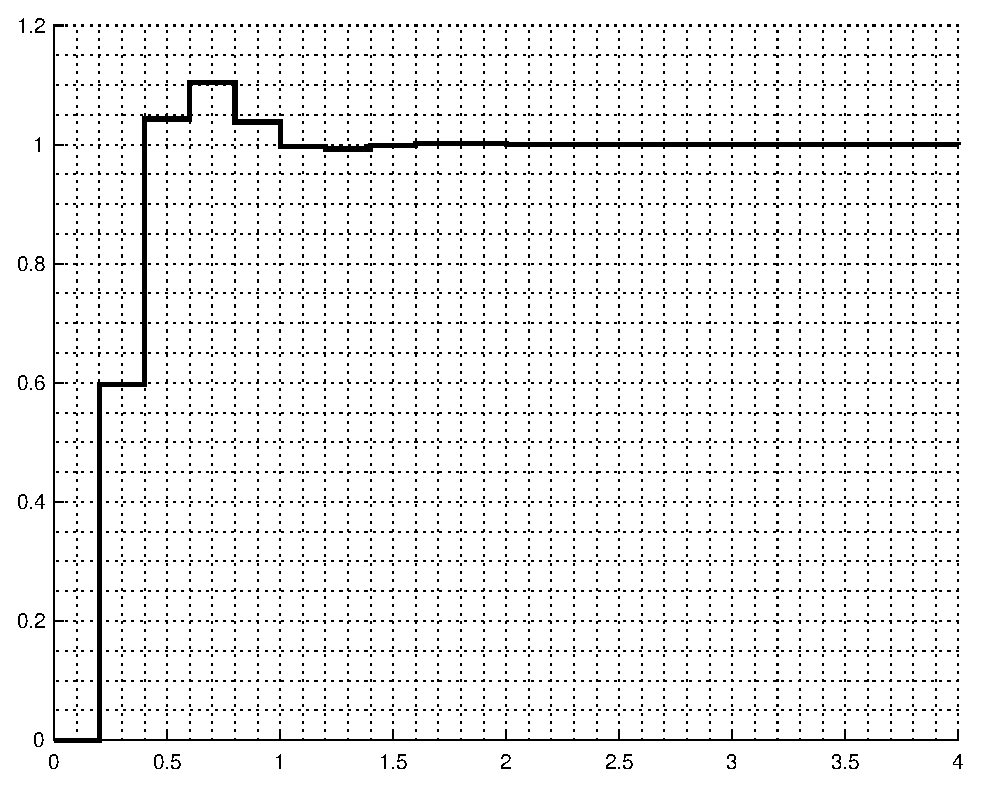
\includegraphics[width=0.75\textwidth]{img/lec6_step4}
%     \caption{PID kontrol için kapalı çevrim basamak yanıtı}
%     \label{fig:lec6_step4}
% \end{figure}

Görüldüğü üzere isterlere oldukça yakın değerler elde edilmiştir. Bunun sebebi, PID kontrolörün fazladan parametreye sahip olması ve bu parametre kullanılarak bir eniyileştirme işleminin mümkün olmasıdır.